\DeclareRobustCommand{\nomenclature}[2]{%
}

\DeclareRobustCommand{\cyrins}[1]{%
 #1
}

\chapter{Применение машинного обучения к ранжированию инцидентов на Московской железной дороге} \label{chapt2}

\section{Введение}
Московская железная дорога (МЖД) \nomenclature{МЖД}{Московская железная дорога} является крупной железнодорожной сетью, включающей в себя 8.8 тыс. км путей и 549 станций. МЖД оснащена несколькими десятками тысяч устройств автоматической регистрации отказов и предотказных состояний оборудования, сигналы которых обрабатываются операторами Центра управления содержанием инфраструктуры. Поток сигналов о возможных инцидентах очень интенсивен и создает большую нагрузку на операторов Центра, причем около 97\% сигналов оказываются ложными тревогами, связанными с недостатками диагностики и техническим обслуживанием оборудования. С целью оптимизации работы Центра нами была разработана основанная на машинном обучении система предварительного автоматического ранжирования инцидентов. Система представляет собой предсказательную модель, оценивающую вероятность наличия реального предотказного состояния по имеющимся признакам сигнала (типа, места, времени,  продолжительности, повторяемости и др.). Предсказательная модель имеет вид ансамбля решающих деревьев, построенного с помощью алгоритма XGBoost по базе данных из 5 миллионов инцидентов. Предсказательная модель внедрена в ПО Центра и используется в повседневной работе операторов.

% \markboth{Journal of \LaTeX\ Class Files,~Vol.~14, No.~8, August~2015}%
% {Shell \MakeLowercase{\textit{et al.}}: Bare Demo of IEEEtran.cls for IEEE Journals}

% \renewcommand{\nomname}{Список сокращений}
% \printnomenclature[5em]

\subsection{Схема работы ЦУСИ}
Московская железная дорога (МЖД) \nomenclature{МЖД}{Московская железная дорога} является крупной железнодорожной сетью, включающей в себя 8.8 тыс. км путей и 549 станций. МЖД оснащена несколькими десятками тысяч устройств ЖАТ (железнодорожная автоматика и телемеханика), производящих автоматическую регистрацию инцидентов -- отказов и предотказных состояний оборудования. Центр управления содержанием инфраструктуры \nomenclature{ЦУСИ}{Центр управления содержанием инфраструктуры} Московской железной дороги (ЦУСИ МЖД) осуществляет непрерывный мониторинг инцидентов на всех участках железной дороги. 
\nomenclature{ЖАТ}{Железнодорожная автоматика и телемеханика}

Инцидент представляет собой совокупность ситуаций, несущих признаки предотказного состояния (например, кратковременное превышение максимально допустимого напряжения оборудования). Наиболее распространенные типы ситуаций, приводящие к предотказам, показаны на рис \ref{fig:histblue}; всего выделяют около 600 различных типов ситуаций. %(уменьшенное время перекрытия стрелки, понижение сопротивления изоляции, пониженное напряжение на путевом реле и т.п.).  

\begin{figure*}
\centering
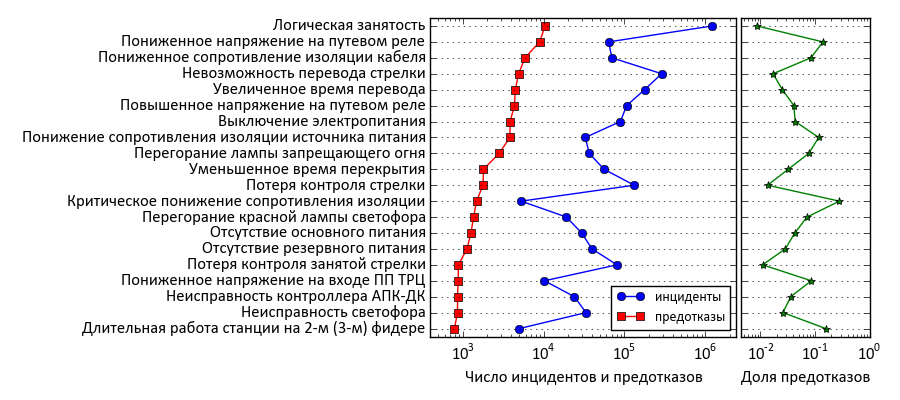
\includegraphics[width=\textwidth]{incidentsvsfaults-lines.png}
% 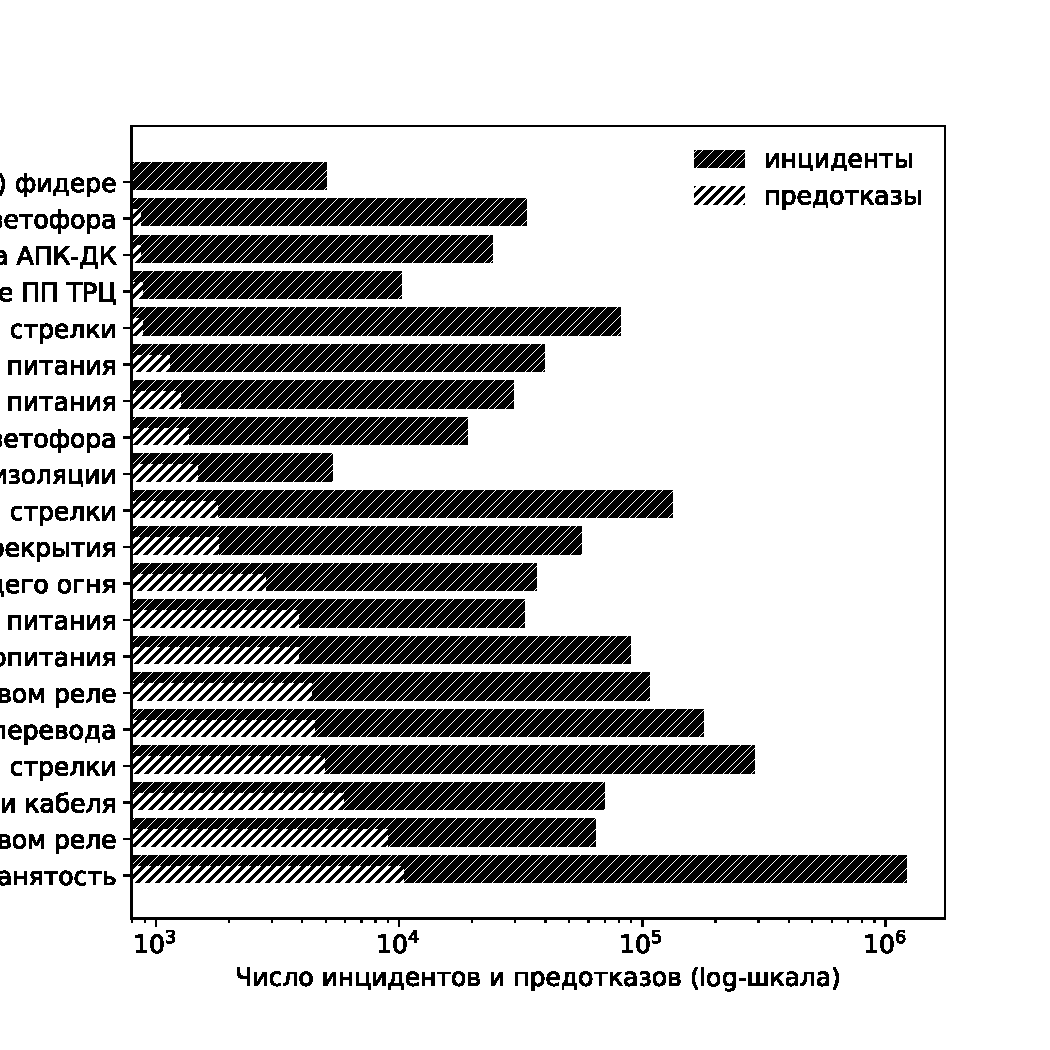
\includegraphics[width=14cm]{incidentsvsfaults-2}
\caption{Наиболее распространённые типы ситуаций, приводящих к предотказу}
\centering
\label{fig:histblue}
\end{figure*}

% \begin{figure*}[t]
% \centering
% 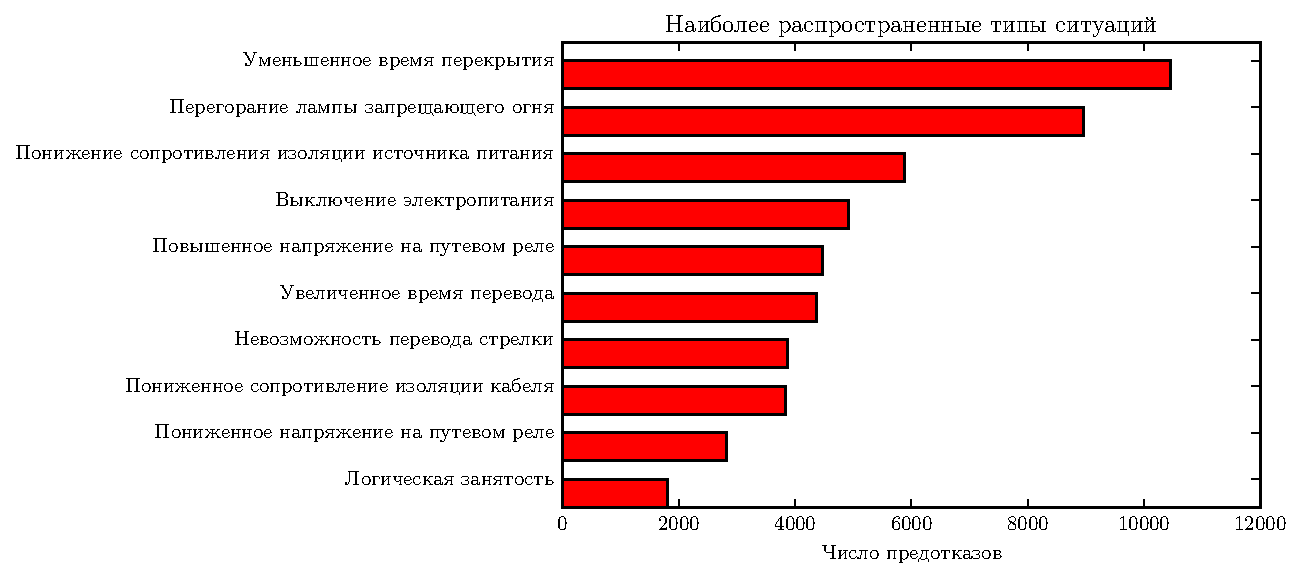
\includegraphics[width=12cm]{redhist}
% \caption{Наиболее распространённые типы ситуаций устройств телемеханики, приводящие к предотказу}
% \centering
% \label{fig:histred}
% \end{figure*}

\begin{figure}[t]
\centering
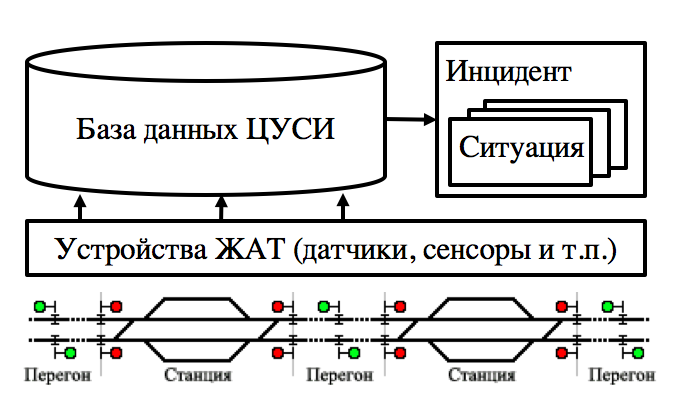
\includegraphics[width=8cm]{arch}
\caption{Последовательность формирования инцидентов: архитектура системы мониторинга}
\centering
\label{fig:arch}
\end{figure}

Ситуации автоматически объединяются в инциденты в базе данных ЦУСИ (см. рис \ref{fig:arch}). Текущие инциденты обрабатываются операторами ЦУСИ, которые выявляют их причины, классифицируют как относящиеся к одному из нескольких типов и принимают необходимые меры. 

Выделяют следующие типы инцидентов (по причине возникновения): предотказное состояние, техническое обслуживание и ремонт, недостатки диагностики и технологическая ситуация. Предотказные состояния образуют наиболее важный тип инцидентов, требующий оперативного реагирования, однако его доля среди всех инцидентов сравнительно невелика (2-3\%). При этом, благодаря достигнутой в последние годы высокой степени обеспечения систем МЖД средствами сбора данных, приходящий в ЦУСИ для обработки операторами поток инцидентов является крайне интенсивным: как правило, новые инциденты могут появляться с интервалом в несколько секунд; общее число инцидентов за 2015 год составило около 1.3 миллионов. 
Таким образом, с точки зрения снижения нагрузки на операторов и повышения эффективности их работы крайне актуальной является задача предварительного автоматического ранжирования инцидентов по степени их важности. В настоящей заметке мы описываем решение этой задачи, полученное нами с помощью методов машинного обучения и внедренное в систему принятия решений ЦУСИ МЖД. 

% \subsection{Постановка задачи}
% \textbf{Задача} состоит в том, чтобы автоматически классифицировать инциденты, регистрируемые устройствами железнодорожной автоматики и телемеханики,  по их признакам на неисправности, ТОиР и т.п. В качестве \textbf{входных данных} могут использоваться все известные на текущий момент параметры инцидента (признаки места, времени, типа события, показания датчиков и т.п.) и его контекст (например, погода, прошлые инциденты и т.п.). \textbf{Выходные данные}: вероятность того, что инцидент связан с предотказом контролируемого объекта (число от 0 до 1).

\section{Постановка задачи и методика решения}
\subsection{Статистический характер задачи}\label{sec:stat}
Отметим, что важность инцидента можно считать определяемой двумя факторами: вероятностью того, что данный инцидент является реальным предотказным состоянием, и последствиями (в частности, экономическим эффектом) данного отказа. Эти два фактора имеют совершенно разный характер и в значительной степени независимы друг от друга. В то время как вероятность предотказного состояния является предметом статистического анализа на основе лишь сохраненных оперативных данных об инцидентах, оценка последствий отказа предполагает привлечение дополнительных стоимостных моделей отказов и других соображений. В настоящей работе мы акцентируем внимание лишь на первом, вероятностном факторе важности; второй фактор учитывается ЦУСИ МЖД отдельно, с помощью нескольких альтернативных моделей.  
С учетом сделанного замечания цель данной работы можно сформулировать как построение прогнозной модели, которая предсказывает вероятность предотказного состояния для данного инцидента на основе автоматически сформированных данных об этом инциденте.


\subsection{Исходные данные}
Каждый \cyrins{\textit{инцидент}} в базе данных ЦУСИ представляет собой набор \cyrins{\textit{ситуаций}} -- единичных событий, несущих признаки предотказного состояния (например, повышение напряжения, понижение сопротивления и т.п.), см. рис. \ref{fig:arch}. Ситуации автоматически объединяются в инциденты на этапе предварительной обработки сигналов датчиков. В простейшем случае инцидент содержит несколько последовательных однотипных ситуаций (например, несколько случаев кратковременного повышения напряжения на одном и том же приборе), но может содержать и разнотипные ситуации, затрагивающие разное оборудование (например, увеличенное время перевода стрелки и некорректные параметры тока перевода). Количество ситуаций в инциденте может варьироваться от одного до нескольких сотен и может увеличиваться со временем, пока инцидент не рассмотрен и не закрыт оператором ЦУСИ. В общей сложности база данных ЦУСИ содержит около 5 млн. инцидентов, включающих 100 млн. ситуаций.  

Описание каждой ситуации содержит ее тип, время начала и окончания, 
ID места (станции или перегона), ID объекта измерения (прибора) и некоторые другие, менее существенные элементы. Большинство свойств (кроме времени) являются категориальными, причем количество их значений может быть достаточно большим: данные охватывают несколько сот типов ситуаций и мест и около 65000 приборов.

При закрытии инцидента оператором ставится пометка о выявленном типе инцидента, в частности являлся ли он предотказом. 

Таким образом, исторические данные содержат достаточно богатую и хорошо структурированную информацию для построения сложных прогностических моделей вероятности предотказа.    

\subsection{Простейшая модель ранжирования}\label{sec:ref_model} 

В качестве примера простой предсказательной модели можно привести прогноз вероятности предотказного состояния исключительно на основе типа первой ситуации инцидента, а именно как долю предотказных инцидентов среди всех наблюдавшихся ранее инцидентов с первой ситуацией данного типа. Это доля сильно зависит от типа ситуации, например, из рис. \ref{fig:histblue} видно, что для ситуации «Критическое понижение сопротивления изоляции» она значительно выше, чем для «Потери контроля занятой стрелки». Поскольку различных типов ситуаций несколько сотен и операторы, очевидно, не в состоянии помнить характеристики каждой из них, даже эта простейшая автоматическая модель ранжирования оказывается практически полезной. В дальнейшем мы будем называть эту модель ``референсной''.  

\subsection{Машинное обучение}
Машинное обучение (МО) \nomenclature{МО}{Машинное обучение} на основе имеющихся исторических данных об инцидентах позволяет строить гораздо более точные предсказательные модели. Стандартная практика машинного обучения \cite{hastie01statisticallearning, Mitchell:1997:ML:541177, scikit-learn} предполагает построение модели в два этапа:
\begin{enumerate}
\item извлечение признаков и формирование обучающей матрицы;
\item применение к полученной обучающей матрице некоторого общего МО-алгоритма.
\end{enumerate}
В ходе первого этапа информация о каждом инциденте приводится к унифицированному виду числового вектора фиксированной размерности, компоненты которого (признаки) отражают потенциально существенные для прогноза характеристики инцидента. Мы описываем этот этап в разделе \ref{sec:feature_extraction}.

В ходе второго этапа к полученной обучающей матрице обычно применяется один из стандартных МО-алгоритмов: логистическая регрессия, нейронные сети, ансамбли решающих деревьев и т.п. Нами использовался алгоритм XGBoost построения ансамбля решающих деревьев с помощью градиентного бустинга \cite{chen2016xgboost}. Мы описываем этот этап в разделе \ref{sec:xgboost}.  

\subsection{Извлечение признаков}\label{sec:feature_extraction}
Извлечение признаков являлось наиболее творческой и трудоемкой частью решения задачи. Оно было связано со следующими трудностями:
\begin{itemize}
\item В общем случае, признаки необходимо агрегировать из всех ситуаций данного инцидента, учитывая, что ситуаций может быть произвольное число. Нами были рассмотрены различные стратегии агрегации, например: ограничиться первой или последней ситуацией в инциденте; в случае числовых признаков взять максимум, минимум или среднее значение по всем ситуациям; в случае категориальных признаков отметить все категории, встреченные в ситуациях инцидентах или сосчитать количество различных встреченных категорий. Конечно, некоторые признаки естественным образом связаны с инцидентом в целом (например, полная продолжительность или место инцидента).
\item Естественным способом преобразования категориального признака с $N$ возможными значениями в числовую форму является его кодирование в виде вектора длины $N$ с единственным ненулевым элементом (one-hot-encoding). Ввиду того, что в рассматриваемой задаче $N$ достигает нескольких сотен или даже тысяч,  обучающие матрицы реализовывались нами в виде разреженных матриц.    
\end{itemize}
С учетом этих обстоятельств, мы рассмотрели несколько десятков различных признаков, описывающих пространственно-временные и прочие характеристики инцидентов. 

Важную роль при создании и отборе признаков играла оценка их значимости, которая осуществлялась нами с помощью двух методов. 
\begin{itemize}
\item
Во-первых, мы оценивали важность признака по общему числу соответствующих ветвлений в итоговой предсказательной модели -- лесе решающих деревьев. Для ``сильно ветвящихся'' признаков мы производили попытку самостоятельно разбить признак на несколько вспомогательных. 
\item Во-вторых, мы реализовали жадный переборный алгоритм последовательного добавления в модель новых признаков, дающих наибольших прирост точности. Этот способ требует многократного обучения модели на различных наборах признаков и поэтому сравнительно долог, однако он позволяет понять, несут ли новые признаки какую-то существенную новую информацию по отношению к уже имеющимся, и какой минимальный набор признаков обеспечивает приемлемую точность модели. Мы подробно описываем результаты этого исследования в разделе \ref{sec:greedy}.
\end{itemize}
Отметим, что помимо признаков, извлекаемых из базы инцидентов, нами была сделана попытка сформировать дополнительные признаки на основе метеоданных, поскольку погодные условия, очевидно, должны оказывать сильное влияние на возникновение некоторых предотказных состояний. Мы действительно обнаружили наличие корреляций между погодными признаками и количеством инцидентов, однако добавление этих признаков в нашу модель не дало заметного улучшения. Иными словами, информация о погоде позволяет улучшить прогноз возникновения инцидента при отсутствии иной информации, но не позволяет заметно улучшить прогноз предотказа при наличии уже имеющейся в базе данных информации об инциденте.


% Отметим следующие наблюдения:
% \begin{itemize}
% \item Как обсуждается далее в разделе \ref{sec:efficiency}, включение в обучающую выборку признаков, родственных уже имеющимся, не дает прироста точности прогноза.
% При этом оказалось довольно эффективным сформировать несколько различных признаков, зависящих лишь от времени (полная продолжительность инцидента, время суток и день недели, максимальная продолжительность ситуаций и др.).
% \item Погодные условия, очевидно, должны оказывать сильное влияние на возникновение некоторых инцидентов. Нами была сделана попытка привлечь метеоданные для улучшения точности предсказательной модели, однако добавление соответствующих признаков не привело к заметному улучшению. С другой стороны, мы действительно наблюдали наличие корреляций между погодными признаками и количеством инцидентов. Иными словами, информация о погоде позволяет улучшить прогноз возникновения инцидента при отсутствии иной информации, но не позволяет заметно улучшить прогноз предотказа при наличии уже имеющейся в базе данных информации об инциденте.  
% \end{itemize}

\subsection{Ансамбль решающих деревьев}\label{sec:xgboost}
Предсказательная модель строилась нами с помощью библиотеки XGboost \cite{chen2016xgboost}. Эта открытая библиотека, хорошо зарекомендовавшая себя в большом числе задач анализа данных\cite{chen2016xgboost}. За последнее время XGBoost неоднократно использовался для решения индустриальных задач, таких как предсказание потребления топлива \cite{horituchi2017predicting}, сбоев технологических процессов (\cite{bosch,DBLP:conf/bigdataconf/Hebert16}), и различных свойств химических составов(\cite{sheridan2016extreme,babajide2016bioactive}). XGboost содержит эффективную реализацию градиентного бустинга \cite{friedman2001greedy}, поддерживающую большие выборки и разреженные матрицы, что было важно в данном проекте. Предсказательная модель представляется в виде суммы ансамбля  бинарных решающих деревьев, последовательно добавляемых в ходе обучения. 

Заметим, что референсная модель из раздела  \ref{sec:ref_model} также естественным образом реализуется в виде ансамбля решающих деревьев, построенных по одному категориальному признаку -- типу первого инцидента. А именно, она состоит из тривиальных деревьев глубины 1 (``решающих пней''), по одному на каждую из компонент бинарного вектора, кодирующего этот категориальный признак. Таким образом, наша основная модель является естественным обобщением референсной модели на случай произвольного набора признаков, числа деревьев и их глубины.

Основная модель была обучена по 3 годам исторических данных (около 5.3 млн. инцидентов) и включала в себя 4000 деревьев глубины 10. Подбор параметров модели осуществлялся стандартным образом с помощью тестирования на контрольной части обучающей выборки.

% \subsection{Признаки инцидентов}\label{sec:feature_extraction}
% Как уже упоминалось, каждый инцидент представляется как набор ситуаций; каждая ситуация характеризуется своим типом, временем и местом проявления, прибором, на котором она наблюдалась, и некоторыми другими сведениями. Ниже приведены основные признаки инцидентов, получаемые на вход при ранжировании. Перед применением алгоритмов машинного обучения, на основании указанных признаков, порождается расширенный набор признаков, описывающие более сложные свойства. 
% Например, 

% Признаки типа и количества ситуаций:
% \begin{enumerate}
% \item Типы всех ситуаций в инциденте
% \item Типы всех отказавших объектов
% \item Тип первой ситуации 
% \item Тип первого отказавшего объекта
% \item Общее количество ситуаций
% \item Количество различных объектов
% \item Количество различных типов ситуаций
% \end{enumerate}

% Признаки времени:
% \begin{enumerate}
% \item Время наступления каждой ситуации инцидента
% \item Время завершения: аналогично
% \item Продолжительность инцидента
% \item Время между первой и второй ситуацией
% \item Время последнего обновления
% \end{enumerate}

% Признаки места:

% \begin{enumerate}
% \item Принадлежность инцидента станции или перегону
% \item Принадлежность дистанции
% \end{enumerate}
% Прочие признаки:

% \begin{enumerate}
% \item «Тревожность» инцидента (экспертная эвристическая оценка)
% \end{enumerate}


%\subsection{Линейная модель, простое решающее правило}



% \subsection{Предлагаемый подход на основе машинного обучения}
% Современные методы машинного обучения позволяют, добиться гораздо большей точности прогноза путем учета большого числа признаков предотказного состояния в рамках сложной логической структуры, массива всех исторических наблюдений. В рамках предложенного подхода была предложена следующая стратегия порождения решающего правила.

% \subsubsection{Подготовка исходных данных}
% Ниже описывается процедура предварительной обработки исходных данных, содержащихся в базе инцидентов.
% \begin{itemize}
% \item Исправление пропусков и некорректных значений. На этом этапе для каждого признака порождается дополнительный признак – индикатор некорректного значения. Для численных признаков значение заменяется средним значением, для категориальных – индикатором пропуска.
% \item Нормализация распределений численных переменных. На этом этапе подбирается трансформация, преобразующая множество значений величины в отрезок [0;1]. 
% \item Текстовые и категориальные признаки бинаризуются, категориальный признак с множеством значений размера N заменяется разреженной матрицей с N+1 столбцами. На практике встречающиеся редко величины признаков принято объединять в один признак. В данной работе такой подход не использовался. Вместо этого производился анализ значимости каждого признака с последующим выбором наиболее важных.
% \end{itemize}

% Параметры соответствующих преобразований над множеством признаков сохраняются индивидуально для каждого признака. Эти преобразования далее применяются повторно при обработке инцидентов в реальном времени.

% \subsubsection{Порождение сложных признаков}
% Самый трудоемкий этап подготовки массива данных – порождение сложных признаков из множества простых, хранящихся в базе данных. При порождении такого рода признаков требуется следить за тем, что аналогичные признаки могли бы быть посчитаны не только по историческому массиву данных, но и в оперативном режиме работы классификатора. 

% \begin{itemize}
% \item Из исходного признака времени порождаются признаки выходных и праздничных дней, времени суток. В качестве независимых признаков выделяются также номера дня в году, месяце и неделе, номер месяца, час, минута и секунда начала инцидента.
% \item Признаки времени и места также дополнялись признаками погодных условий – давление, температура, влажность и скорость ветра.
% \item Признаки территориальной принадлежности (номер дистанции, номер объекта) дополняются кластеризующими признаками. В нашем случае для кластеризации удалось воспользоваться номером объекта в базе данных (объекты в базе нумеруются последовательно с внедрением и неявно несут информацию о времени и месте установки).
% \item Признаки, характеризующие частоту поступления инцидентов для того или иного типа объекта ЖАТ (стрелки, светофоры, рельсовые цепи) для разных временных промежутков (от 1 минуты до месяца). Аналогичные составные признаки были выделены для различных мест обнаружения инцидентов (станция, перегон и т.д.).
% \end{itemize}

% \subsubsection{Исследование важности порожденных признаков}
% Заключительный этап подготовки данных заключается в проверке статистической значимости переменных в модели. Этот шаг выполняется, чтобы отбросить шумящие переменные. Для оценки значимости признаков в данной работе использовалось два подхода.

% Первый подход заключается в исследовании поведения показателя AUC при добавлении нового признака на вход обучаемого классификатора. В этом случае для ускорения расчетов мы используем заниженное значение количества раундов обучения и жадный алгоритм выбора очередного признака. Более важным признаком будем считать такой признак, при добавлении которого достигается максимальное увеличение площади под операционной характеристикой классификатора. Эффективность каждого отдельного признака показана на \ref{fig:initialFeatureScores}. На рисунке \ref{fig:adaptiveAdditionScores} можно увидеть последовательное изменение величины показателя AUC при добавлении новых признаков. На рисунке \ref{fig:featureHeatmap} показано насколько больший прирост дает добавляемый признак по сравнению с еще не добавленными.

% Второй подход заключается в изучении количественных характеристик итогового решающего правила (леса решающих деревьев) на всем множестве признаков после прохода раундов обучения. В этом случае более важным признаком будем считать такой признак, которому соответствует большее суммарное количество разветвлений в итоговом решающем правиле. Для "сильно ветвящийся" признаков мы производили попытку самостоятельно разбить признак на несколько вспомогательных.

% \begin{figure*}
% \centering
% 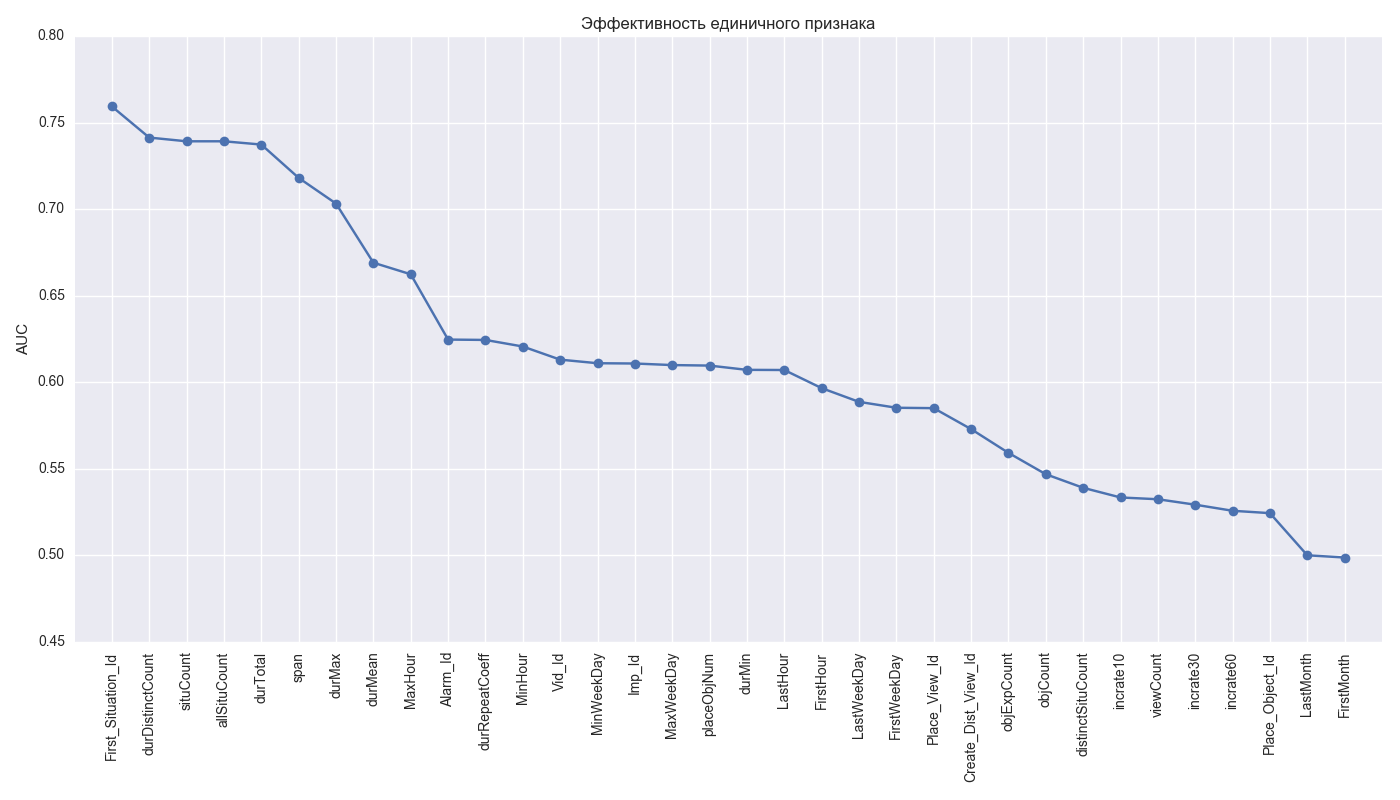
\includegraphics[width=6cm]{initialFeatureScores}
% \caption{Анализ важности признаков: эффективность отдельных признаков}
% \centering
% \label{fig:initialFeatureScores}
% \end{figure*}



% \begin{figure*}
% \centering
% 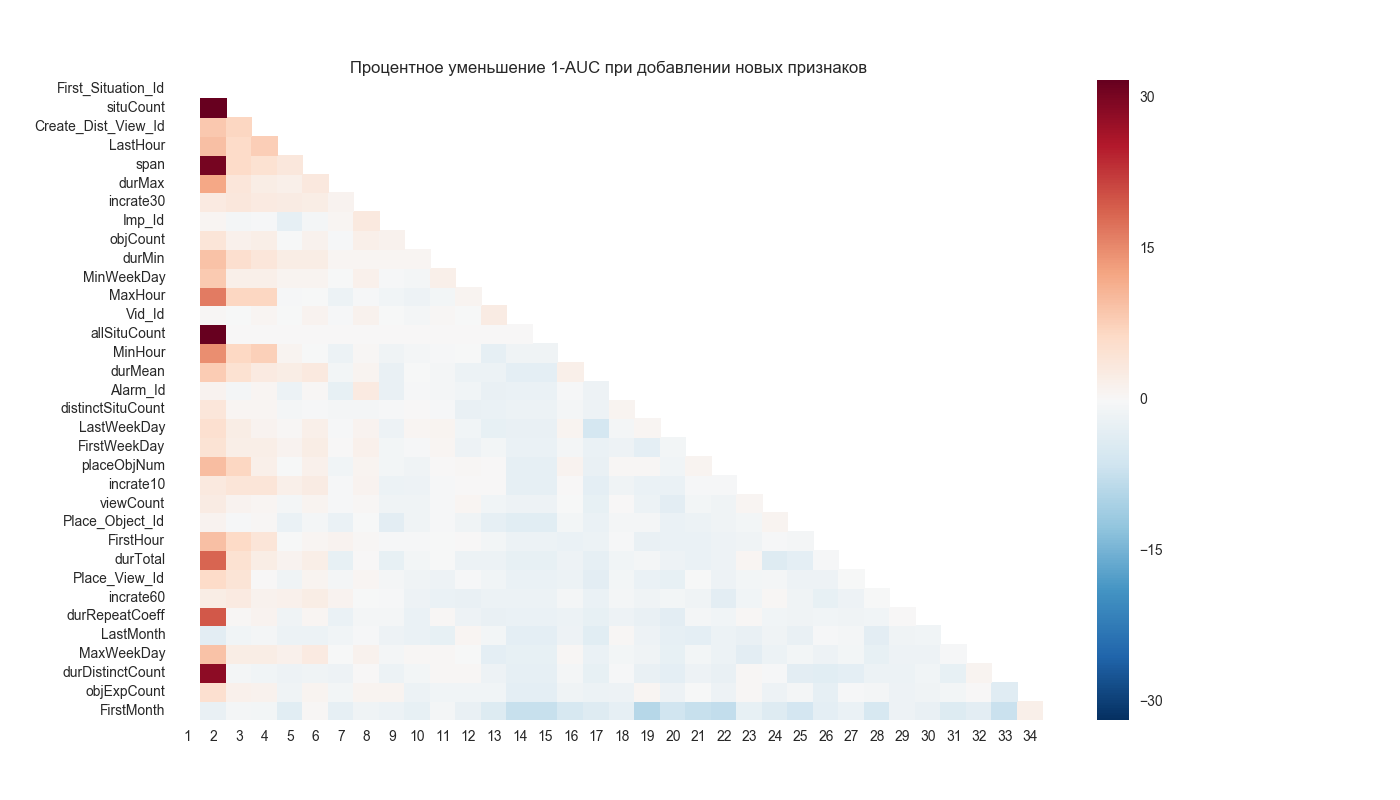
\includegraphics[width=16cm]{featureHeatmap}
% \caption{Анализ важности признаков: последовательное добавление}
% \centering
% \label{fig:featureHeatmap}
% \end{figure*}

% \subsubsection{Настройка параметров обучения}
% Перед настройкой параметров алгоритма исходная выборка инцидентов разделяется на обучающую и контрольную подвыборки. Выбор параметров обучения производится по следующей стратегии.
% На начальном этапе при помощи скользящего контроля по тестовой выборке выбирается количество решающих деревьев (\textit{n\_estimators}). Между оптимальными значениями скорости обучения (eta) и количеством решающих деревьев (\textit{n\_estimators}) существует естественная зависимость – чем ниже скорость обучения, тем больше деревьев необходимо, чтобы достичь максимальной точности. После выбора достаточно высокой скорости обучения (0.1 – 0.2) мы итеративно увеличиваем количество деревьев, пока падает ошибка кросс-валидации и переходим к следующему этапу. На следующем этапе подстраиваются параметры решающих деревьев, ответственные за контроль переобучения: \textit{max\_depth}, \textit{min\_child weight}, \textit{gamma}. На последнем этапе производим обучение классификатора с меньшей скоростью обучения (0.025 – 0.1).

% \subsubsection{Характеристики решающего правила}
% Построенная нами высокоточная прогнозная модель имеет вид ансамбля глубоких решающих деревьев \cite{friedman2001greedy} 
% включает в себя 4000 деревьев глубины 10. Пример одного дерева показан на рис. \ref{fig:tree}.

% \begin{figure}
% \centering
% 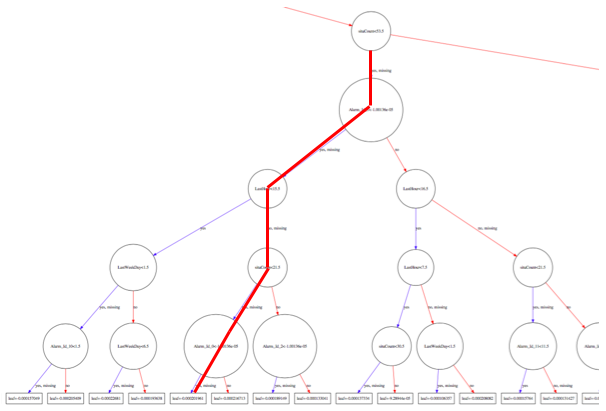
\includegraphics[width=5.5cm]{gr_path}
% \caption{Пример прохода по решающему дереву: Если в инциденте: а) количество ситуаций меньше 53, б) последняя ситуация произошла позже 15:30
% и в) тревожность равна 1, то повысить вероятность предотказа.
% }
% \centering
% \label{fig:tree}
% \end{figure}

% Пример цепочки решающих правил, отвечающих проходу по одной ветви дерева, показан на рис. 5. Окончательный прогноз вероятности предотказа получается усреднением прогнозов по всем деревьям.  

\section{Анализ модели}

%\pagecolor{yellow!30!orange}
\begin{figure}[thpb] 
\centering
% \includegraphics[width=7cm]{histo2}
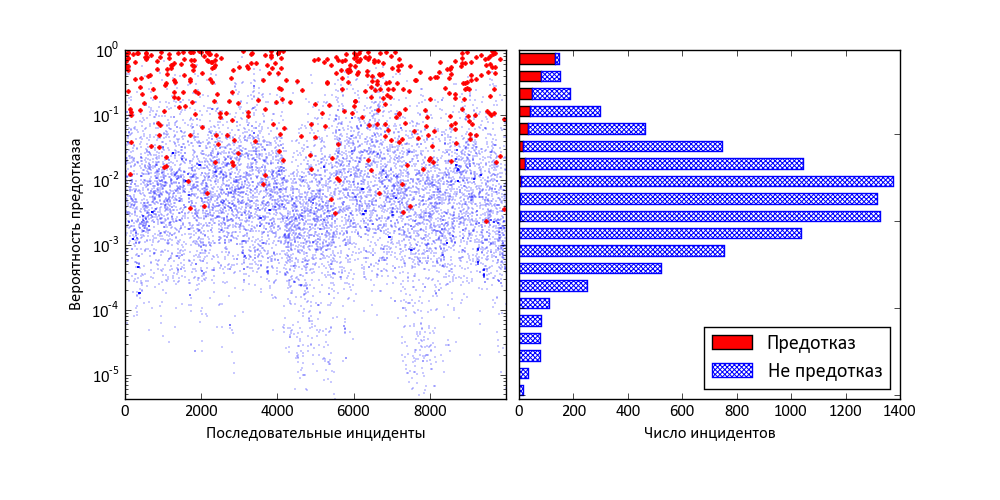
\includegraphics[trim=7mm 7mm 11mm 5mm, clip, width=\textwidth]{threswall-plus.png}
\caption{Результаты ранжирования 10000 последовательных инцидентов.  Предотказы показаны крупными точками, ложные тревоги -- мелкими. В правой части рисунка показаны соответствующие гистограммы распределения инцидентов по вероятности.}
\centering
\label{fig:histo}
\end{figure}


\subsection{Тестовое ранжирование}

В соответствии со стандартной практикой машинного обучения, тестирование построенной модели проводилось на тестовой выборке, изолированной от обучающей выборки, причем обучающие инциденты предшествовали по времени тестовым. 

На рисунке \ref{fig:histo} приведены результаты ранжирования 10000 последовательных инцидентов. Крупные точки показывают инциденты, связанные с предотказами, а мелкие -- инциденты, связанные с ложными срабатываниями системы. Хорошо видно, что основная масса предотказов имеет высокую вероятность и визуально отделена по вероятности от основной массы ложных тревог, имеющей меньшую вероятность. Это свидетельствует о пригодности использования предсказательной модели в качестве ранжирующей функции.

Из рисунка очевидна некоторая неравномерность и периодичность распределения вероятности предотказа в зависимости от номера инцидента. Этот эффект объясняется суточным циклом (показанные 10000 инцидентов отвечают временному интервалу продолжительностью около 3 дней). В дневное время значительное число инцидентов связано с техническим обслуживанием и ремонтом; модель присваивает низкую вероятность предотказа таким инцидентам.


% Следует отметить, что существенная доля предотказов имеет после классификации значение вероятности в промежутке 0.001 и 0.1. Для удобства восприятия, это значение выводится на экран инженера службы мониторинга в логарифмической шкале. На рисунке 6 представлена гистограмма распределения значения ранга после логарифмического преобразования. Видно, что большинство инцидентов, связанных с предотказами, находится в промежутке 0.5 – 1.0. 

\subsection{Количественные оценки эффективности ранжирования}
Для количественной оценки эффективности ранжирования мы используем кривую ошибок, определяемую следующим образом. Предположим, что операторы успевают обрабатывать лишь некоторую долю всех инцидентов; рассмотрим соответствующую переменную ДОИ (Доля Обработанных Инцидентов) со значениями в интервале $[0,1]$. Будем считать, что операторы в первую очередь обрабатывают те инциденты, для которых модель предсказывает наиболее высокую вероятность отказа. Пусть величина ДОО (Доля Охваченных Отказов), также со значениями в интервале $[0,1]$, обозначает долю обрабатываемых при этом предотказных инцидентов среди всех предотказных инцидентов. Кривая ошибок тогда представляет собой график зависимости ДОО от ДОИ.

\nomenclature{AUC}{Area Under Curve (англ.), площадь под кривой ошибок}
\nomenclature{ДОИ}{Доля обработанных инцидентов}
\nomenclature{ДОО}{Доля охваченных отказов} 

\begin{figure}[thb] 
\begin{center}
\begin{subfigure}[c]{0.45\textwidth}
        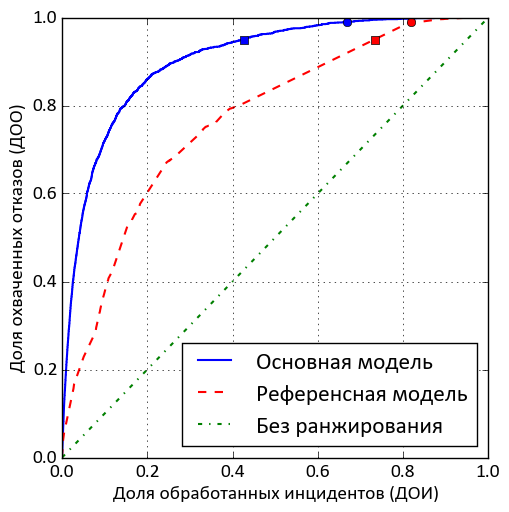
\includegraphics[width=1\linewidth]{latexRoc.png}
\end{subfigure}
%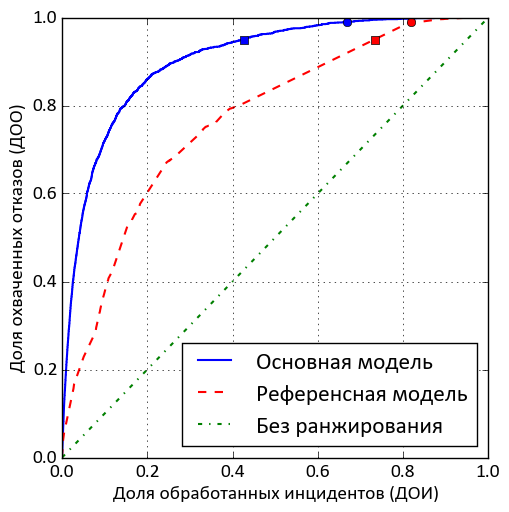
\includegraphics[width=0.5\linewidth]{latexRoc}
\begin{subfigure}[c]{0.45\textwidth}
\begin{tabular}{ l c c c}
\toprule
\cyrins{\textbf{Модель}} & \cyrins{\textbf{AUC}} & \cyrins{\textbf{ДОИ95\%}} & \cyrins{\textbf{ДОИ99\%}} \\ \midrule
Основная & 0.904& 0.427 & 0.669 \\
Референсная & 0.768 & 0.733 & 0.818\\
\bottomrule
\end{tabular}
\end{subfigure}
\caption{Кривые ошибок и связанные с ними характеристики для основной и референсной моделей. Выделенные точки отвечают ДОО 0.95 и  0.99.}\label{fig:ROCcurves} 
\end{center}
\end{figure}

На рис. \ref{fig:ROCcurves} показаны кривые ошибок для основной и референсной моделей ранжирования. Чем выше лежит кривая, тем лучше. Максимально возможное положение кривой соответствует линейной функции $\text{ДОО}=\frac{ДОИ}{\alpha},$ где $\alpha\approx 0.024$ -- доля предотказов среди всех инцидентов. Если оператор выбирает инцидент наугад (без рассмотрения ранга), то кривая ошибок является диагональю квадрата.

В качестве основной количественной характеристики точности мы рассматриваем AUC (Area Under Curve) -- площадь под кривой ошибок. Ее значения для обеих моделей приведены в таблице на рис. \ref{fig:ROCcurves}. Кроме того, мы приводим значения ДОИ95\% и ДОИ99\%, которые определяются как те значение ДОИ, при которых ДОО составляет, соответственно, 0.95 и 0.99. Заметим, в частности, что если операторы обрабатывают лишь половину инцидентов, а именно те, которые имеют основной ранг выше медианного значения, то при этом пропускается менее 5\% предотказных состояний.


\begin{figure*}[thpb] 
\begin{center}
\begin{subfigure}[c]{\textwidth}\caption{Динамика точности ранжирования и ее прироста.}
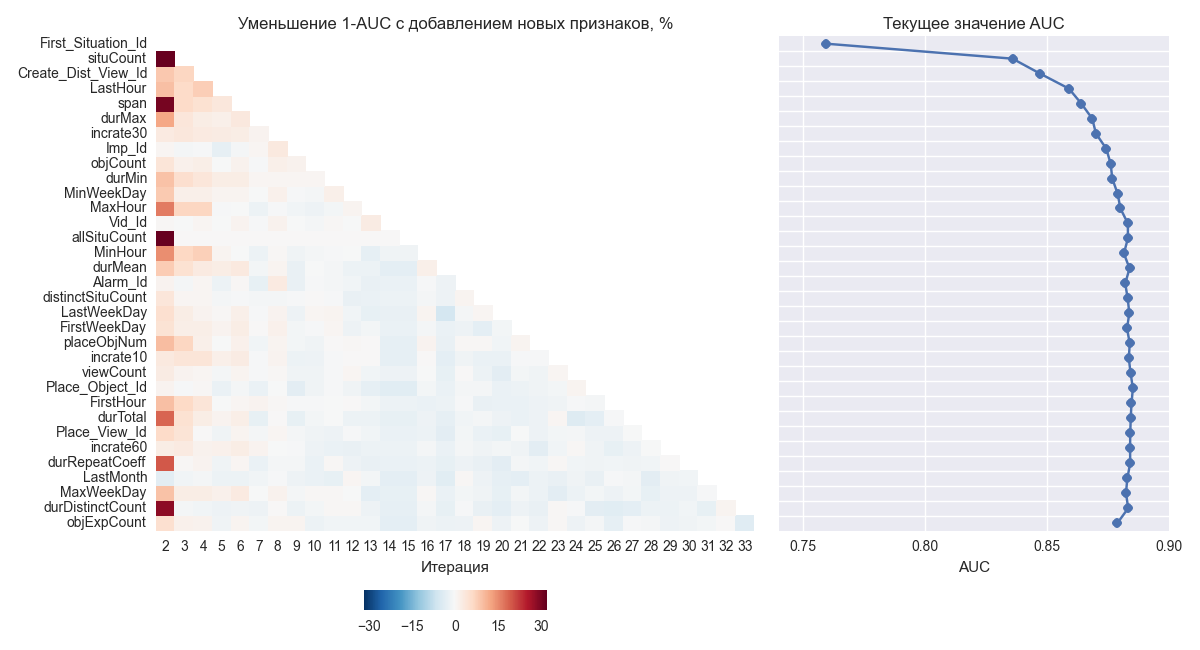
\includegraphics[width=\linewidth]{fullAdaptiveData.png}
\end{subfigure}\\
\begin{subfigure}[c]{\textwidth}\caption{Наиболее эффективные признаки, в порядке включения в модель.}\small
\begin{tabular}{ l p{7cm} l}
  \toprule
  \cyrins{\textbf{Признак}} & \cyrins{\textbf{Описание}} & \cyrins{\textbf{Тип, число значений}} \\ 
  \midrule
  {\texttt First\_Situation\_id} & Тип первой ситуации в инциденте & Категориальный, $\sim$600\\ 
  {\texttt situCount} & Количество ситуаций в инциденте & Количественный\\ 
  {\texttt Create\_Dist\_View\_id} & Дистанция (место) инцидента & Категориальный, 22  \\  
  {\texttt LastHour} & Час последней ситуации в инциденте & Количественный \\ 
  {\texttt span} & Продолжительность инцидента от начала первой до начала последней ситуации & Количественный \\ 
  {\texttt durMax} & Максимальная продолжительность ситуации в инциденте & Количественный \\ 
%   {\texttt Place\_Object\_Id} & Идентификатор отказавшего объекта, на котором возникла первая ситуация   & Категориальный, $\sim$65000  \\
  {\texttt incrate30} & Количество инцидентов, зарегистрированных на объекте %{\texttt Place\_Object\_Id} 
  в пределах 30 мин до регистрации инцидента  & Количественный  \\
  {\texttt imp\_id} & Степень важности инцидента & Категориальный, 4 \\
  {\texttt objCount} & Количество объектов, затронутых инцидентом & Количественный \\
  {\texttt durMin} & Минимальная продолжительность ситуации в инциденте & Количественный\\
  {\texttt MinWeekDay} & Минимальное значение дня недели 
  среди ситуаций инцидента & Категориальный, 7  \\
%   {\texttt MaxHour} & Максимальное значение часовой компоненты 
%   среди ситуаций инцидента & Категориальный, 24 \\
%   {\texttt Vid\_id} & Идентификатор вида инцидента & Категориальный \\
  \bottomrule
\end{tabular}
\end{subfigure}
\caption{Анализ важности признаков с помощью их последовательного жадного добавления. На каждой итерации к текущему набору признаков, начиная с {\texttt First\_Situation\_id}, добавляется новый признак, при котором точность ранжирования увеличивается сильнее всего. (a)  На диаграмме слева показаны относительные изменения величины $1-\textrm{AUC}$ при добавлении каждого из признаков, не входящих в текущий набор. График справа показывает динамику точности предсказательной модели, построенной по текущему набору признаков. (b) Несколько первых признаков, до насыщения модели.}\label{fig:adaptiveAdditionScores}
\end{center}
\end{figure*}

\subsection{Анализ эффективности признаков}\label{sec:greedy}
На рис. \ref{fig:adaptiveAdditionScores} показаны результаты эксперимента по последовательному адаптивному добавлению в модель новых признаков. На каждом шаге для каждого из еще не входящих в модель признаков совершается пересчет точности модели с этим дополнительным признаком; тот, для которого наблюдается наибольшее приращение точности, включается в модель. В общей сложности рассматривается 34 признака, процедура начинается с признака типа первой ситуации (как наиболее информативного). 

В левой части рисунка \ref{fig:adaptiveAdditionScores}(a) показаны относительные изменения характеризующей ошибку величины $1-\text{AUC}$ для каждой итерации (горизонтальная ось) и каждого признака--кандидата (вертикальная ось). Признаки упорядочены post factum по очередности включения в модель, так что диаграмма имеет треугольный вид. В правой части рисунка показаны значения AUC соответствующей модели для каждой итерации. Для ускорения процедуры, модели в этом эксперименте строились с уменьшенным числом деревьев, поэтому их значения AUC ниже значения, указанного для основной модели на рис. \ref{fig:ROCcurves}. 

В результате данного эксперимента мы видим, что модель насыщается после включения в нее 10 -- 15 признаков, и ее точность перестает существенно меняться, если не считать небольшого эффекта переобучения, наблюдаемого в конце эксперимента. Первые несколько признаков являются одновременно достаточно информативными и разнообразными; их описания приведены в таблице \ref{fig:adaptiveAdditionScores}(b). На левой части рис. \ref{fig:adaptiveAdditionScores}(a) хорошо видно, что полезность признаков падает с итерациями, причем падение является резким в моменты, когда в набор включается признак, родственный рассматриваемому (см., например, \texttt{span} и \texttt{situCount}). Несмотря на это, мы видим, что полезно иметь, например, много разных признаков, характеризующих время ситуаций.

\nomenclature{АПК-ДК}{Аппаратно-программный комплекс диспетчерского контроля}

\begin{figure}[thb] 
\centering
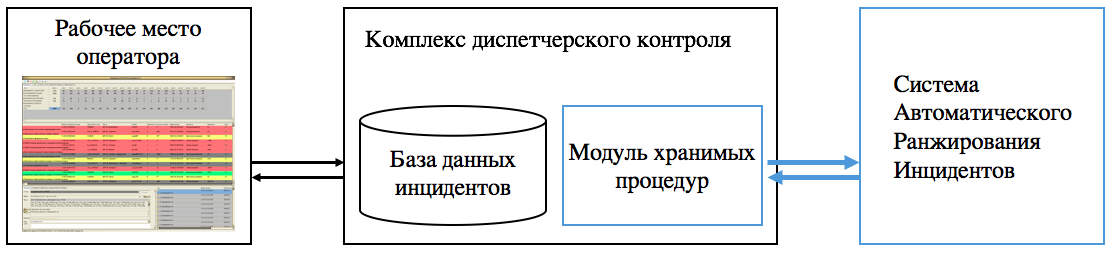
\includegraphics[width=13cm]{modules-v2}
\centering
\caption{Схема интеграции САРИ и АПК ДК.}
\centering
\label{fig:modules}
\end{figure}

\begin{figure*}[thb] 
\centering
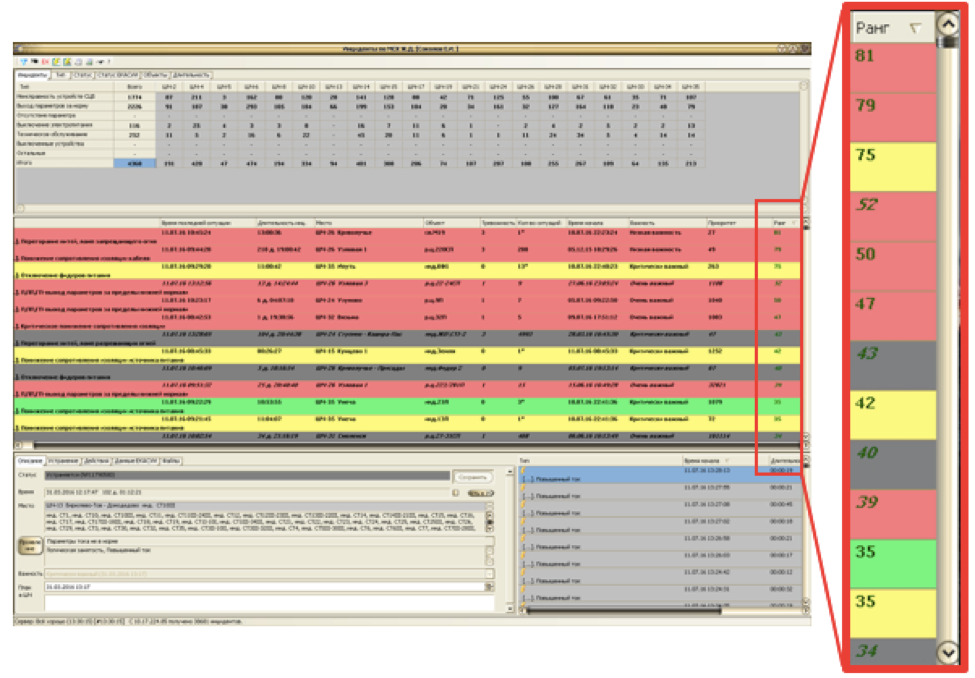
\includegraphics[width=11cm]{ui}
\caption{Отображение результатов ранжирования в пользовательском интерфейсе инженера службы мониторинга.}
\centering
\label{fig:ui}
\end{figure*}

\nomenclature{АРМ}{Автоматизированное рабочее место}

\section{Опыт внедрения}
Построенная модель ранжирования инцидентов была интегрирована в виде нового элемента, АПК «САРИ» (Система автоматического ранжирования инцидентов), в комплекс диспетчерского контроля ЦУСИ РЖД. \nomenclature{САРИ}{Система автоматического ранжирования инцидентов}  Схема интеграции и взаимодействующие модули представлены на рис. \ref{fig:modules}. 

Модуль ранжирования инцидентов выполняется на изолированном сервере. Он синхронно опрашивает модуль хранимых процедур в базе данных инцидентов на предмет обновления полей инцидентов и при необходимости инициирует пересчет при получении новых инцидентов и ситуаций. Важно отметить, что не все поля данных могут быть получены в оперативном режиме.

При получении новых данных, модуль осуществляет ранжирование инцидентов по набору исходных признаков и выдает прогнозное значение. Это значение далее отображается в виде отдельного столбца в интерфейсе инженера службы мониторинга с возможностью сортировки, см. рис. \ref{fig:ui}. Предсказательная модель выдает обновленное ранжирующее значение за 1.2 миллисекунды. Для удобства восприятия операторами, ранги инцидентов выдаются в виде целых чисел из интервала $[0,100]$ и соответствуют интервалу вероятностей $[10^{-6},1]$ на логарифмической шкале.


% На исторических данных построено решающее правило, лес из 4000 решающих деревьев глубины 10.  Итоговое правило имеет 300,549 вариантов исходов и включает в себя более 3 лет исторических данных (5.3 млн инцидентов).

За время подконтрольной эксплуатации системы (май--июнь 2016 года, 1 месяц) в ней было зарегистрировано 581 032 ситуаций, объединенных в 92 339 инцидентов. Среди них предотказами было признано 2187 инцидентов. %Среднее время ответа САРИ – 1.7 мс. 
Точность модели в тестовой эксплуатации оказалась очень близка к предварительной оценке на тестовой выборке (AUC 0.901 и 0.904, соответственно).

% \begin{figure}
% \centering
% 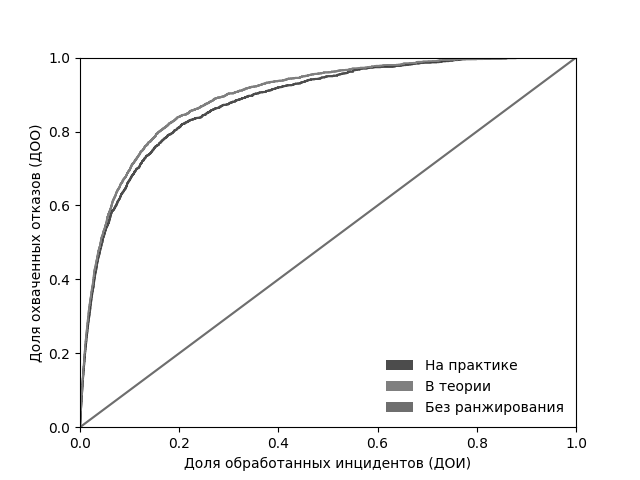
\includegraphics[width=9cm]{image19}
% \caption{Операционная характеристика функции ранжирования (в теории и на практике)}
% \centering
% \label{fig:image19}
% \end{figure}

% На практике была показан режим работы, при котором для захвата 80\% предотказов достаточно охватить 20\% общей массы инцидентов в системе. Оценка снижения времени реакции инженера мониторинга на предотказ - до 5 раз (см. Рис. \ref{fig:ROCcurves}).

% Модель полезно периодически обновлять, чтобы учитывать свежие данные. На графике ниже показано улучшение при обновлении раз в квартал.



\section{Обсуждение}
Нами была разработана и внедрена основанная на машинном обучении модель автоматического ранжирования инцидентов, регистрируемых устройствами ЖАТ на Московской железной дороге. Модель позволяет инженерам Центра управления инфраструктурой оперативно оценивать вероятности отказов и предотказных состояний и сокращает время реакции и устранения неполадок. Нами продемонстрирована высокая точность ранжирования с помощью построенной модели. Нам представляется полезным и перспективным более широкое внедрение предложенной нами технологии в системах железнодорожного мониторинга.  

Отметим два возможных направления развития данного проекта. Во-первых, как обсуждалось в разделе \ref{sec:stat}, разработанная нами модель является чисто статистической и не учитывает различия в важности разных отказов и предотказных состояний. Было бы полезно дополнить нашу модель достаточно точной программной моделью потерь как функции отказа. Математически это можно выразить следующим образом. Имеющаяся модель оценивает условную вероятность отказа или предотказного состояния при наличии инцидента с определенными характеристиками: $\mathbb P(\text{предотказ}|\text{инцидент})$. Практически более полезной была бы оценка условного математического ожидания потерь (например, в денежном выражении) при наличии данного инцидента: $\mathbb E(\text{потери}|\text{инцидент})$. Если считать, что потери происходят только при предотказе, то $\mathbb E(\text{потери}|\text{инцидент})=\mathbb E(\text{потери}|\text{предотказ})\cdot\mathbb P(\text{предотказ}|\text{инцидент})$, то есть для оценки $\mathbb E(\text{потери}|\text{инцидент})$ нам необходимо перемножить разработанную нами оценку вероятности предотказа на ожидаемые потери в случае предотказа, $\mathbb E(\text{потери}|\text{предотказ})$. Оценка этой последней величины может быть либо задана явно в соответствии с существующими регламентами, либо, при наличии хорошо структурированных и достаточно полных исторических данных о потерях, получена посредством их анализа с помощью методов, аналогичных применявшимся в настоящей работе.

Другим возможным направлением развития проекта является более глубокий анализ инцидентов, возможно с привлечением более детальной информации о предотказных ситуациях. Имеющаяся в основной исторической базе данных информация об инцидентах часто довольно скудна, например если инцидент состоит лишь из одной ситуации, описывающей повышение напряжения, то вся доступная информация об этом событии ограничивается указанием соответствующего временного интервала. В то же время можно ожидать, что дополнительная информация, скажем, о максимальном значении напряжения, скорости его изменения и т.п., позволила бы уточнить прогноз наличия предотказного состояния.


% Опыт применения методов машинного обучения к задачам управления инфраструктурой российских железных дорог на Московской железной дороге позволяет ожидать положительные практические результаты при дальнейшем развитии и тиражировании достигнутых с совместной рабочей группой специалистов Московской дирекции инфраструктуры Московской железной дороги научных и практических успехов.

% При дальнейшем развитии системы вести в xgboost-модель дополнительные признаки, отражающие историю аналогичных инцидентов/ситуаций на данном участке.

% По результатам данной работы, ученый совет ОАО «РЖД» признал перспективным применение современных методов машинного обучения к задачам управления инфраструктурой российских железных дорог и порекомендовал продолжить развитие, разработку и внедрение системы. 

% Представленные наработки в области интеллектуального анализа данных также рекомендовано апробировать в других областях железнодорожного транспорта.

% \appendix
% \section{Приложение А: Таблица сокращений}
% \begin{tabular}{ p{1.5cm} p{6cm} }
%   \toprule
%   ЦУСИ & Центр управления содержанием инфраструктуры \\ \midrule
%   ЖАТ & Железнодорожная автоматика и телемеханика \\ \midrule
%   САРИ & Система автоматического ранжирования инцидентов \\ \midrule 
%   МЖД & Московская железная дорога \\ \midrule
%   АРМ & Автоматизированное рабочее место \\ \midrule
%   AuC & Area under Curve (англ.), площадь под кривой операционной характеристики классификатора \\ \midrule
%   ДОИ & Доля обработанных инцидентов \\ \midrule
%   ДОО & Доля охваченных отказов \\ \midrule
%   АПК-ДК & Аппаратно-программный комплекс диспетчерского контроля \\ \bottomrule
% \end{tabular}

%\nocite{*}
% \bibliographystyle{bib/utf8gost705u}  %% стилевой файл для оформления 
% \bibliography{bib/bibliography}